\documentclass[fleqn]{article}
\usepackage{amsmath}
\usepackage{graphicx}
\usepackage[utf8]{inputenc}
\newcommand{\myvec}[1]{\ensuremath{\begin{pmatrix}#1\end{pmatrix}}}
\title{Assignment 1}
\author{D V K M Rishab, AI20MTECH14004}
\date{September 5, 2020}
\begin{document}
\let\vec\mathbf
\maketitle
\section*{Assignment 1}
Solution: 
\newline \newline
$\vec{P}$ = \myvec{7\\6} \newline \newline \newline
$\vec{Q}$ = \myvec{3\\4} \newline \newline \newline
A \hspace{0.1cm} vector \hspace{0.1cm} on \hspace{0.1cm} the \hspace{0.1cm} X-axis \hspace{0.1cm} $\vec{X}$ \hspace{0.1cm} is \hspace{0.1cm} equidistant \hspace{0.1cm} to \hspace{0.1cm} both \hspace{0.1cm} $\vec{P}$ \hspace{0.1cm} and \hspace{0.1cm} $\vec{Q}$. \newline \newline
Need \hspace{0.1cm} to \hspace{0.1cm} find \hspace{0.1cm} k. \newline \newline
Let \hspace{0.1cm} $\vec{X}$ = k\myvec{1\\0} \hspace{0.1cm} be \hspace{0.1cm} the \hspace{0.1cm} vector \hspace{0.1cm} on \hspace{0.1cm} the \hspace{0.1cm} X-axis.\newline
\begin{flalign*}
& \implies \myvec{1 & 0} \hspace{0.1cm} \vec{X} = k \\
& \implies \vec{X} = \frac{{\vec{P}+\vec{Q}}}{2} \\ \\
& \implies \vec{X} = \frac{\myvec{7\\6}+\myvec{3\\4}}{2} \\ \\
& \implies \vec{X} = \myvec{5\\5} \\ \\
& \implies \myvec{1 & 0}\vec{X} = \myvec{1 & 0}\myvec{5\\5} \\
& \implies k = 5 \hspace{0.3cm} i.e. \hspace{0.3cm} \vec{X} = \myvec{5\\0}
\end{flalign*}
\section*{Plot}
\begin{figure}[!htb]
    \centering
    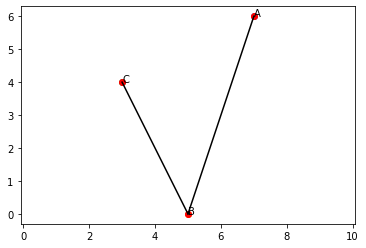
\includegraphics{Assignment1.png}
    \caption{Plot representing the Points}
    \label{Fig.1}
\end{figure}
\end{document}
